%iffalse
\let\negmedspace\undefined
\let\negthickspace\undefined
\documentclass[journal,12pt,onecolumn]{IEEEtran}
\usepackage[version=4]{mhchem}
\usepackage{chemformula} % for \ch if needed
\usepackage{chemfig}
\usepackage{chemmacros}
\chemsetup{modules = reactions} % Enables reaction arrows
\usepackage{graphicx}
\graphicspath{ {./images/} }
\usepackage{geometry}
\usepackage{lastpage}
\usepackage{cite}
\usepackage{amsmath,amssymb,amsfonts,amsthm}
\usepackage{enumitem,multicol}
\usepackage{algorithmic}
\usepackage{graphicx}
\usepackage{textcomp}
\usepackage{xcolor}
\usepackage{txfonts}
\usepackage{listings}
\usepackage{enumitem}
\usepackage{mathtools}
\usepackage{gensymb}
\usepackage{comment}
\usepackage[breaklinks=true]{hyperref}
\usepackage{tkz-euclide} 
\usepackage{listings}
\usepackage{gvv}                                        
%\def\inputGnumericTable{}                                 
\usepackage[latin1]{inputenc}                                
\usepackage{color}                                            
\usepackage{array}                                            
\usepackage{longtable}                                       
\usepackage{calc}                                             
\usepackage{multirow}                                         
\usepackage{hhline}                                           
\usepackage{ifthen}                                           
\usepackage{lscape}
\usepackage{tabularx}
\usepackage{array}
\usepackage{float}


\newtheorem{theorem}{Theorem}[section]
\newtheorem{problem}{Problem}
\newtheorem{proposition}{Proposition}[section]
\newtheorem{lemma}{Lemma}[section]
\newtheorem{corollary}[theorem]{Corollary}
\newtheorem{example}{Example}[section]
\newtheorem{definition}[problem]{Definition}
\newcommand{\BEQA}{\begin{eqnarray}}
\newcommand{\EEQA}{\end{eqnarray}}
\newcommand{\define}{\stackrel{\triangle}{=}}
\theoremstyle{remark}

\geometry{margin=1 in}



\setlength{\headheight}{14pt}
\setlength{\headsep}{5pt}
\setlength{\footskip}{20pt}
\begin{document}
\begin{enumerate}
  
\item The Lewis acidity of \(\mathrm{BF_3}\) is less than \(\mathrm{BCl_3}\) even though fluorine is more electronegative than chlorine. It is due to\\

\hfill{GATE 2010 CY}
\begin{multicols}{2}
\begin{enumerate}
    \item stronger \(2p(\mathrm{B})\)-\(2p(\mathrm{F})\) \(\sigma\)-bonding
    \item stronger \(2p(\mathrm{B})\)-\(2p(\mathrm{F})\) \(\pi\)-bonding
    \item stronger \(2p(\mathrm{B})\)-\(3p(\mathrm{Cl})\) \(\sigma\)-bonding
    \item stronger \(2p(\mathrm{B})\)-\(3p(\mathrm{Cl})\) \(\pi\)-bonding
\end{enumerate}
\end{multicols}
\item Pyroxenes are a class of silicate minerals, which exhibit a polymeric chain structure.\\
Its simplest repeat unit is

\hfill{GATE 2010 CY}

\begin{multicols}{2}
\begin{enumerate}
    \item  $\mathrm{[SiO_4]^{4-}}$
    \item  $\mathrm{[SiO_3]^{2-}}$
    \item  $\mathrm{[Si_2O_7]^{6-}}$
    \item  $\mathrm{[Si_4O_{11}]^{6-}}$
\end{enumerate}
\end{multicols}
\item Among the following pentachlorides the one which does not exist due to the 'inert-pair effect' is
\hfill{GATE 2010 CY}
\begin{multicols}{2}
\begin{enumerate}
    \item PCl$_5$
    \item BiCl$_5$
    \item SbCl$_5$
    \item AsCl$_5$
\end{enumerate}
\end{multicols}

\item Band theory predicts that magnesium is an insulator. However, in practice it acts as a conductor due to
\hfill{GATE 2010 CY}
\begin{multicols}{2}
\begin{enumerate}
    \item presence of filled 3s orbital
    \item overlap of filled 2p and filled 3s orbital
    \item overlap of filled 3s and empty 3p orbital
    \item presence of unfilled 3p orbital
\end{enumerate}
\end{multicols}

\item The number of 'framework electron pairs' present in the borane cluster [B$_{12}$H$_{12}$]$^{2-}$ is

\hfill{GATE 2010 CY}
\begin{multicols}{2}
\begin{enumerate}
    \item 10
    \item 11
    \item 12
    \item 13
\end{enumerate}
\end{multicols}

\item The reaction between [PdCl$_4$]$^{2-}$ and C$_2$H$_4$ produces a new compound. Compared to free C$_2$H$_4$, the C-C bond order of the product is
\hfill{GATE 2010 CY}
\begin{multicols}{2}
\begin{enumerate}
    \item between 1 and 2
    \item less than 1
    \item unaltered
    \item greater than 2
\end{enumerate}
\end{multicols}

\item Among the following pair of metal ions present in Nature, the first one functions as an electron-transfer agent and the second one catalyzes the hydrolysis reactions. The correct pair is
\hfill{GATE 2010 CY}
\begin{multicols}{2}
\begin{enumerate}
    \item Fe and Zn
    \item Mg and Fe
    \item Co and Mo
    \item Ca and Cu
\end{enumerate}
\end{multicols}

\item Structurally nickelocene is similar to ferrocene. Nickelocene attains stability due to the formation of
\hfill{GATE 2010 CY}
\begin{multicols}{2}
\begin{enumerate}
    \item a monocation
    \item a dication
    \item a monanion
    \item a dianion
\end{enumerate}
\end{multicols}
\item The absolute configurations for compounds X and Y, respectively, are
\hfill{GATE 2010 CY}
\begin{figure}[H]
    \centering
    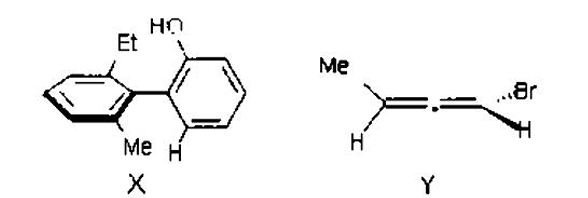
\includegraphics[width=0.5\linewidth]{figs/Q.9.png}
    \caption{fig1}
    \label{fig:figs/Q.9.png}
\end{figure}

\begin{multicols}{2}
\begin{enumerate}
    \item $R,\,S$
    \item $S,\,R$
    \item $R,\,R$
    \item $S,\,S$
\end{enumerate}
\end{multicols}
\item in the reaction
\begin{figure}[H]
    \centering
    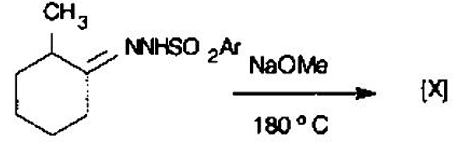
\includegraphics[width=0.5\linewidth]{figs/Q.10.1.png}
    \caption{fig2}
    \label{fig:figs/Q.10.1.png}
\end{figure}
the major product [X] is
\hfill{GATE 2010 CY}
\begin{figure}[H]
    \centering
    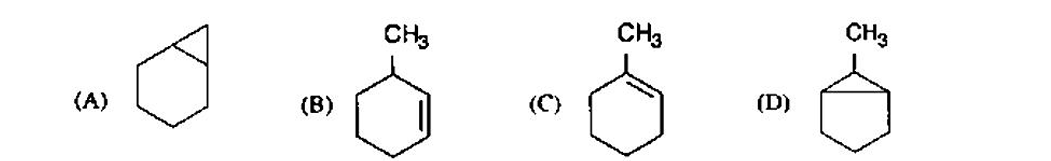
\includegraphics[width=0.75\linewidth]{figs/Q.10.2.png}
    \caption{fig3}
    \label{fig:figs/Q.10.2.png}
\end{figure}
\item Among the following, a pair of resolvable configurational enantiomers is given by

\hfill{GATE 2010 CY}

\begin{multicols}{2}
\begin{enumerate}
    \item \textit{cis}-1,2-dimethylcyclohexane
    \item \textit{cis}-1,3-dimethylcyclohexane
    \item \textit{cis}-1,4-dimethylcyclohexane
    \item \textit{trans}-1,3-dimethylcyclohexane
\end{enumerate}
\end{multicols}
\item in the reaction
\begin{figure}[H]
    \centering
    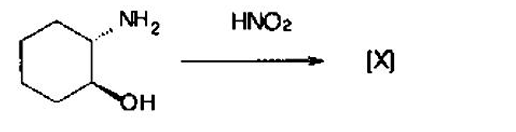
\includegraphics[width=0.5\linewidth]{figs/Q.12.png}
    \caption{fig4}
    \label{fig:figs/Q.12.png}
\end{figure}
the major product [X] is

\hfill{GATE 2010 CY}
\begin{figure}[H]
    \centering
    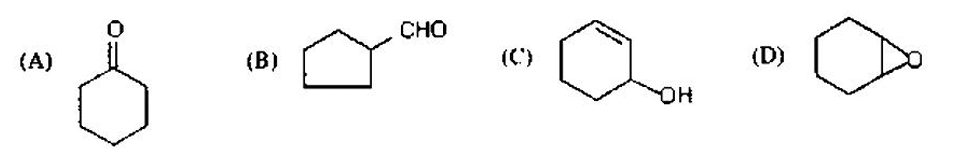
\includegraphics[width=0.75\linewidth]{figs/Q.12.1.png}
    \caption{fig5}
    \label{fig:figs/Q.12.1.png}
\end{figure}
\item The decreasing order of isoelectric point for the following $\alpha$-amino acids is\\
\textbf{Lysine} \hspace{1em} (I) \hspace{3em} \textbf{Alanine} \hspace{1em} (II) \hspace{3em} \textbf{Glutamic acid} \hspace{1em} (III)
\hfill{GATE 2010 CY}

\begin{multicols}{2}
\begin{enumerate}
    \item I $>$ II $>$ III
    \item II $>$ I $>$ III
    \item III $>$ I $>$ II
    \item I $>$ III $>$ II
\end{enumerate}
\end{multicols}

\item The decreasing order of the reactivity of the following compounds towards electrophiles is\\
I \hspace{3em} II \hspace{3em} III


\begin{figure}[H]
    \centering
    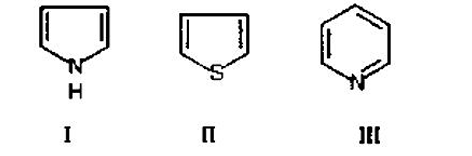
\includegraphics[width=0.5\linewidth]{figs/Q.13.png}
    \caption{fig6}
    \label{fig:figs/Q.13.png}
\end{figure}
\hfill{GATE 2010 CY}

\begin{multicols}{2}
\begin{enumerate}
    \item II $>$ I $>$ III
    \item II $>$ III $>$ I
    \item III $>$ I $>$ II
    \item I $>$ II $>$ III
\end{enumerate}
\end{multicols}

\item 
In the reaction
\begin{figure}[H]
    \centering
    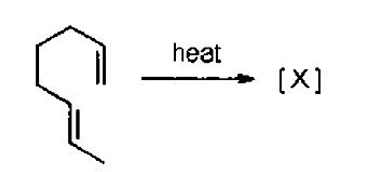
\includegraphics[width=0.5\linewidth]{figs/Q.15.png}
    \caption{fig7}
    \label{fig:figs/Q.15.png}
\end{figure}
the major product [x ] is

\hfill{GATE 2010 CY}
\begin{figure}[H]
    \centering
    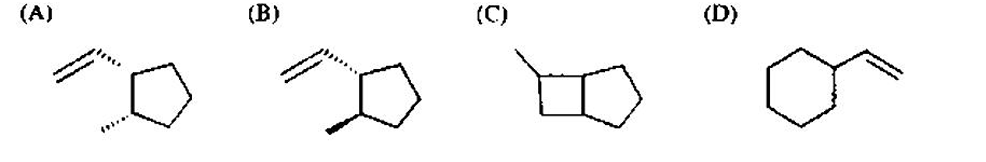
\includegraphics[width=0.75\linewidth]{figs/Q.15.1.png}
    \caption{fig8}
    \label{fig:figs/Q.15.1.png}
\end{figure}
\item The decreasing order of acidity of the marked H of the following molecules is\\
\begin{figure}[H]
    \centering
    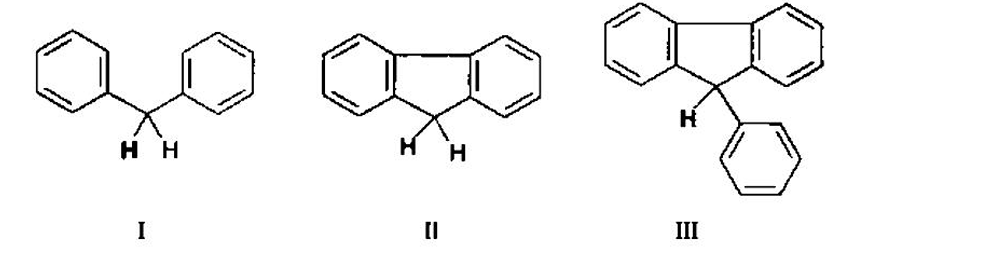
\includegraphics[width=0.5\linewidth]{figs/Q.16.png}
    \caption{fig9}
    \label{fig:figs/Q.16.png}
\end{figure}

\hfill{GATE 2010 CY}

\begin{multicols}{2}
\begin{enumerate}
    \item I $>$ II $>$ III
    \item III $>$ I $>$ II
    \item III $>$ II $>$ I
    \item II $>$ I $>$ III
\end{enumerate}
\end{multicols}
\item The decreasing order of nucleophilicity for the following anions is\\
CH$_3$CO$_2^-$, CH$_3$O$^-$, C$_6$H$_5$O$^-$, NO$_3^-$
\hfill{GATE 2010 CY}

\begin{multicols}{2}
\begin{enumerate}
    \item CH$_3$CO$_2^-$ $>$ CH$_3$O$^-$ $>$ C$_6$H$_5$O$^-$ $>$ NO$_3^-$
    \item CH$_3$O$^-$ $>$ NO$_3^-$ $>$ C$_6$H$_5$O$^-$ $>$ CH$_3$CO$_2^-$
    \item CH$_3$O$^-$ $>$ C$_6$H$_5$O$^-$ $>$ CH$_3$CO$_2^-$ $>$ NO$_3^-$
    \item C$_6$H$_5$O$^-$ $>$ CH$_3$O$^-$ $>$ NO$_3^-$ $>$ CH$_3$CO$_2^-$
\end{enumerate}
\end{multicols}

\item The molar entropy of crystalline CO at absolute zero is
\hfill{GATE 2010 CY}

\begin{multicols}{2}
\begin{enumerate}
    \item Zero
    \item $-\mathrm{R}\ln2$
    \item $\mathrm{R}\ln2$
    \item $2\mathrm{R}\ln2$
\end{enumerate}
\end{multicols}

\item For an ideal gas
\begin{multicols}{2}
\begin{enumerate}
    \item $(\partial P/\partial T)_V\,(\partial T/\partial V)_P\,(\partial V/\partial P)_T = 0$
    \item $(\partial P/\partial T)_V\,(\partial T/\partial V)_P\,(\partial V/\partial P)_T = -1$
    \item $(\partial P/\partial T)_V\,(\partial T/\partial V)_P\,(\partial V/\partial P)_T = +1$
    \item $(\partial P/\partial T)_V\,(\partial T/\partial V)_P\,(\partial V/\partial P)_T = +2$
\end{enumerate}
\end{multicols}

\item Among W (work), Q (heat), U (internal energy) and S (entropy)

\begin{multicols}{2}
\begin{enumerate}
    \item W and U are path functions but Q and S are state functions
    \item W and S are path functions but Q and U are state functions
    \item S and U are path functions but Q and W are state functions
    \item W and Q are path functions but U and S are state functions
\end{enumerate}
\end{multicols}

\item For eigen functions $\psi_1 = \sqrt{\frac{1}{b}} \sin\left(\frac{\pi x}{b}\right)$ and $\psi_2 = \sqrt{\frac{2}{b}} \sin\left(\frac{2\pi x}{b}\right)$ of particle in a 1-D box of length $b$ ($0 \leq x \leq b$)
\begin{multicols}{2}
\begin{enumerate}
    \item $\psi_1$ is normalized and orthogonal to $\psi_2$
    \item $\psi_1$ is normalized but not orthogonal to $\psi_2$
    \item $\psi_2$ is normalized and orthogonal to $\psi_1$
    \item $\psi_2$ is neither normalized nor orthogonal to $\psi_1$
\end{enumerate}
\end{multicols}

\item The bond order of C$_2$ molecule is
\hfill{GATE 2010 CY}
\begin{multicols}{2}
\begin{enumerate}
    \item 0
    \item 1
    \item 2
    \item 3
\end{enumerate}
\end{multicols}
\item Sulfur can exist in four phases. The possible number of triple points is
\hfill{GATE 2010 CY}

\begin{multicols}{2}
\begin{enumerate}
    \item 1
    \item 2
    \item 3
    \item 4
\end{enumerate}
\end{multicols}

\item The standard reduction potentials at 298 K for single electrodes are given below:\\

\begin{tabular}{l l}
\textbf{Electrode} & \textbf{Electrode Potential (volt)} \\
Mg$^{2+}$ / Mg & $-2.34$ \\
Zn$^{2+}$ / Zn & $-0.76$ \\
Fe$^{2+}$ / Fe & $-0.44$ \\
\end{tabular}

From this we can infer that

\hfill{GATE 2010 CY}

\begin{multicols}{2}
\begin{enumerate}
    \item Zn can reduce both Mg$^{2+}$ and Fe$^{2+}$
    \item Fe can reduce both Mg$^{2+}$ and Zn$^{2+}$
    \item Mg can reduce both Zn$^{2+}$ and Fe$^{2+}$
    \item Mg can reduce Zn$^{2+}$ but not Fe$^{2+}$
\end{enumerate}
\end{multicols}
\item For the pair of reactions given below

\begin{itemize}
    \item[i)] $\mathrm{N_2(g) + 3H_2(g) \rightleftharpoons 2NH_3(g)}$
    \item[ii)] $\mathrm{\frac{1}{2}N_2(g) + \frac{3}{2}H_2(g) \rightleftharpoons NH_3(g)}$
\end{itemize}

If at a particular temperature, $K_{P1}$ and $K_{P2}$ are the equilibrium constants for reactions i) and ii) respectively, then

\begin{multicols}{2}
\begin{enumerate}
    \item $K_{P1} = 2K_{P2}$
    \item $K_{P1} = K_{P2}^2$
    \item $2K_{P1} = K_{P2}$
    \item $K_{P1}^2 = K_{P2}$
\end{enumerate}
\end{multicols}
26-55 Carry two marks each
\item According to VSEPR model, the shape of [XeOF$_5$]$^-$ is
\hfill{GATE 2010 CY}

\begin{multicols}{2}
\begin{enumerate}
    \item octahedral
    \item trigonal bipyramidal
    \item square pyramidal
    \item pentagonal monopyramidal
\end{enumerate}
\end{multicols}

\item The number of unpaired electron(s) present in the species [Fe(H$_2$O)$_5$(NO)]$^{2+}$ which is formed during 'brown ring test' is
\hfill{GATE 2010 CY}

\begin{multicols}{2}
\begin{enumerate}
    \item 2
    \item 3
    \item 4
    \item 5
\end{enumerate}
\end{multicols}

\item Fe$_3$O$_4$ and Co$_3$O$_4$ are metal oxides having spinel structure. Considering their CFSEs, the correct statement regarding their structure is
\hfill{GATE 2010 CY}

\begin{multicols}{2}
\begin{enumerate}
    \item both have normal spinel structure
    \item both have inverse spinel structure
    \item Fe$_3$O$_4$ has normal and Co$_3$O$_4$ has inverse spinel structure
    \item Fe$_3$O$_4$ has inverse and Co$_3$O$_4$ has normal spinel structure
\end{enumerate}
\end{multicols}

\item The mechanism of the reaction between [Fe(CN)$_6$]$^{4-}$ and [Fe(bpy)$_3$]$^{3+}$ (bpy = 2,2$'$-bipyridine) is
\hfill{GATE 2010 CY}

\begin{multicols}{2}
\begin{enumerate}
    \item outer-sphere electron-transfer
    \item inner-sphere electron-transfer
    \item self-exchange reaction
    \item ligand exchange followed by electron transfer
\end{enumerate}
\end{multicols}
\item The d-d absorption band of [Fe(H$_2$O)$_6$]$^{2+}$ is split due to
\hfill{GATE 2010 CY}

\begin{multicols}{2}
\begin{enumerate}
    \item presence of octahedral geometry
    \item static Jahn-Teller distortion
    \item dynamic Jahn-Teller distortion
    \item presence of trigonal bipyramidal geometry
\end{enumerate}
\end{multicols}

\item The crystal-field symbol for the ground-state of [Mn(CN)$_6$]$^{4-}$ is
\hfill{GATE 2010 CY}

\begin{multicols}{2}
\begin{enumerate}
    \item $^2T_{2g}$
    \item $^1A_{1g}$
    \item $^3E_g$
    \item $^4A_{1g}$
\end{enumerate}
\end{multicols}

\item In the following reactions, the reagent/conditions X and Y are
\hfill{GATE 2010 CY}
\begin{figure}
    \centering
    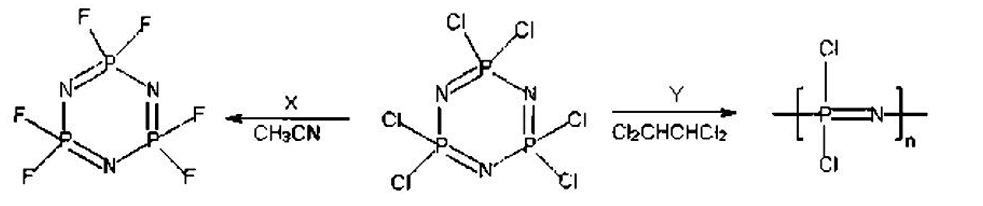
\includegraphics[width=0.5\linewidth]{figs/Q.32.png}
    \caption{fig10}
    \label{fig:figs/Q.32.png}
\end{figure}

\begin{multicols}{2}
\begin{enumerate}
    \item X = BF$_3$; Y = heating at 125$^\circ$C
    \item X = NaF; Y = heating at 250$^\circ$C
    \item X = NH$_4$F; Y = HCl
    \item X = CF$_3$SO$_3$H; Y = H$_2$SO$_4$
\end{enumerate}
\end{multicols}

\item 
is a blue coloured complex. Controlled-treatment of this complex with water generates two isomeric light pink coloured complexes of composition [Co(H$_2$O)$_4$Cl$_2$]. Identify the correct point groups for [CoCl$_4$]$^{2-}$ and two isomeric complexes [Co(H$_2$O)$_4$Cl$_2$].

\begin{multicols}{2}
\begin{enumerate}
    \item $D_{4h}$ and ($C_{2v}$ and $C_{2h}$)
    \item $T_d$ and ($C_{2v}$ and $D_{4h}$)
    \item $D_{4h}$ and ($C_{2v}$ and $D_{4h}$)
    \item $T_d$ and ($C_{2v}$ and $C_{4v}$)
\end{enumerate}
\end{multicols}
\item 
in the reaction
\begin{figure}[H]
    \centering
    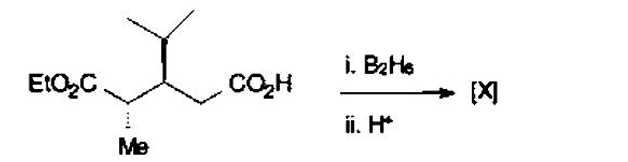
\includegraphics[width=0.5\linewidth]{figs/Q.34.png}
    \caption{fig11}
    \label{fig:figs/Q.34.png}
\end{figure}
the major product [x] is
\hfill{GATE 2010 CY}
\begin{figure}[H]
    \centering
    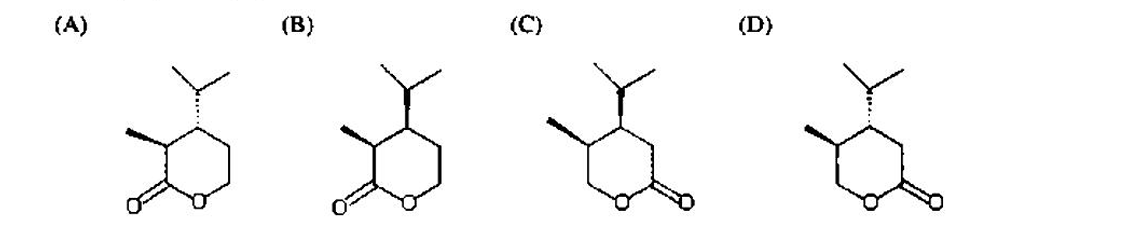
\includegraphics[width=0.75\linewidth]{figs/Q.35.1.png}
    \caption{Enter Caption}
    \label{fig:placeholder}
\end{figure}
\item 
In the reaction 
\begin{figure}[H]
    \centering
    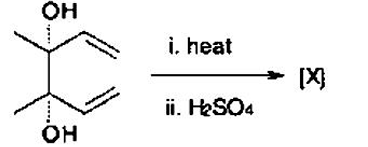
\includegraphics[width=0.5\linewidth]{figs/Q.35.png}
    \caption{fig13}
    \label{fig:figs/Q.35.png}
\end{figure}
\hfill{GATE 2010 CY}
\begin{figure}[H]
    \centering
    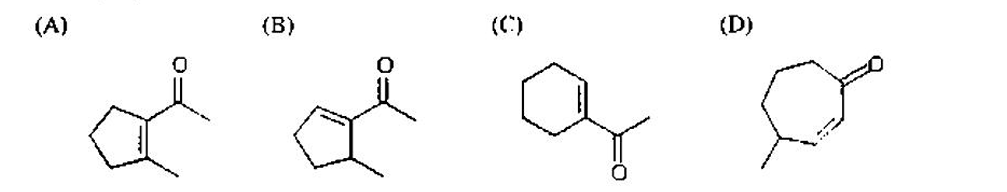
\includegraphics[width=0.75\linewidth]{figs/Q.35.2.png}
    \caption{fig14}
    \label{fig:figs/Q.35.2.png}
\end{figure}
\item 
in the following sequence
\begin{figure}[H]
    \centering
    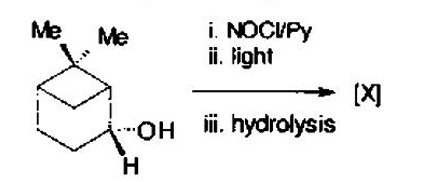
\includegraphics[width=0.5\linewidth]{figs/Q.36.png}
    \caption{fig15}
    \label{fig:figs/Q.36.png}
\end{figure}
the major product [X] is
\hfill{GATE 2010 CY}
\begin{figure}[H]
    \centering
    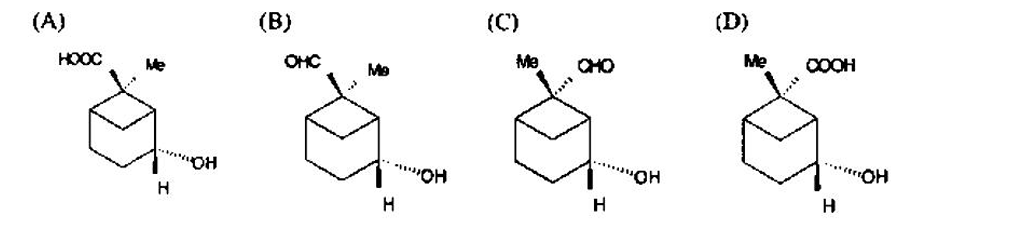
\includegraphics[width=0.75\linewidth]{figs/Q.36.1.png}
    \caption{fig16}
    \label{fig:figs/Q.36.1.png}
\end{figure}
\item 
In the reaction
\begin{figure}[H]
    \centering
    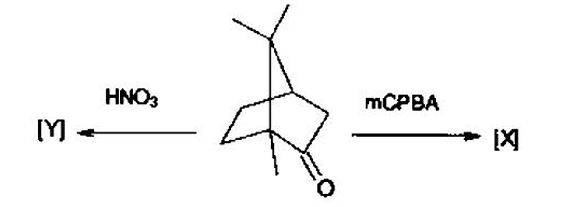
\includegraphics[width=0.5\linewidth]{figs/Q.17.png}
    \caption{fig17}
    \label{fig:figs/Q.17.png}
\end{figure}
the major produc [x] is
\hfill{GATE 2010 CY}
\begin{figure}[H]
    \centering
    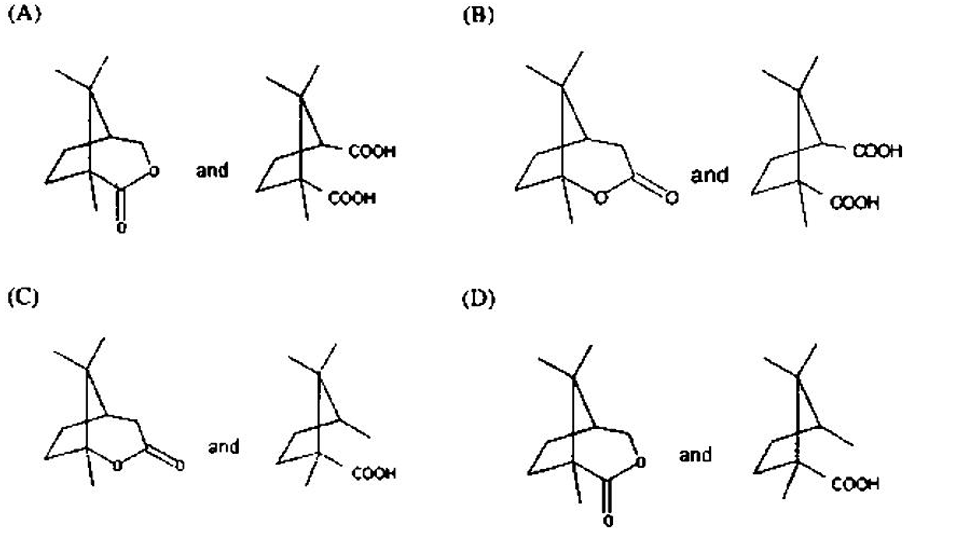
\includegraphics[width=0.75\linewidth]{figs/Q.37.1.png}
    \caption{fig18}
    \label{fig:figs/Q.37.1.png}
\end{figure}
\item 
in the reaction
\begin{figure}[H]
    \centering
    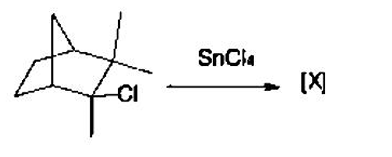
\includegraphics[width=0.5\linewidth]{figs/Q.38.png}
    \caption{fig19}
    \label{fig:figs/Q.38.png}
\end{figure}
\hfill{GATE 2010 CY}
the major PRODUCT [x] is
\begin{figure}[H]
    \centering
    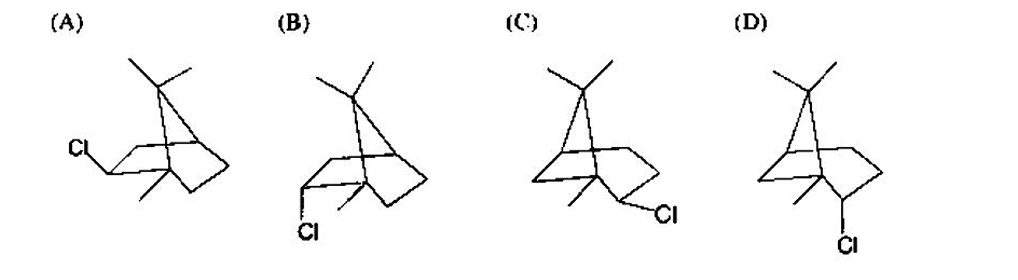
\includegraphics[width=0.80\linewidth]{figs/Q.38.1.png}
    \caption{fig20}
    \label{fig:figs/Q.38.1.png}
\end{figure}
\item in the reaction
\begin{figure}[H]
    \centering
    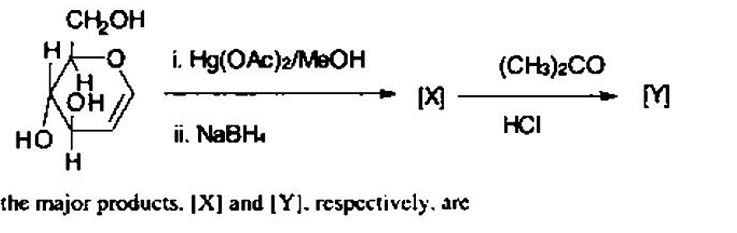
\includegraphics[width=0.75\linewidth]{figs/Q.39.png}
    \caption{fig21}
    \label{fig:figs/Q.39.png}
\end{figure}
\hfill{GATE 2010 CY}
\begin{figure}[H]
    \centering
    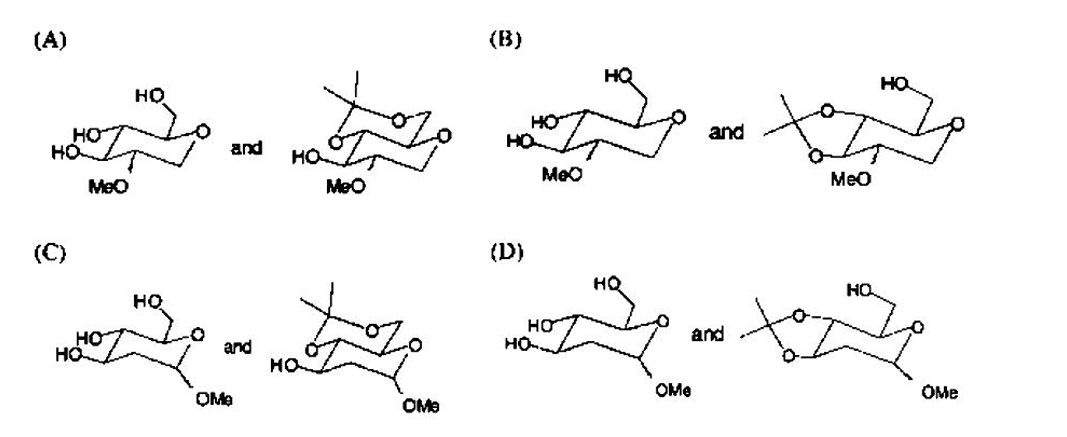
\includegraphics[width=1\linewidth]{figs/Q.39.1.png}
    \caption{fig22}
    \label{fig:figs/Q.39.1.png}
\end{figure}
\item The change in entropy when two moles of Argon gas are heated at constant volume from 300 K to 500 K is
\hfill{GATE 2010 CY}

\begin{multicols}{2}
\begin{enumerate}
    \item $-12.74~\mathrm{J~K^{-1}~mole^{-1}}$
    \item $-6.37~\mathrm{J~K^{-1}~mole^{-1}}$
    \item $6.37~\mathrm{J~K^{-1}~mole^{-1}}$
    \item $12.74~\mathrm{J~K^{-1}~mole^{-1}}$
\end{enumerate}
\end{multicols}

\item At any temperature $T$, the fugacity coefficient $(\gamma)$ is given by

\[
\ln \gamma = \int_0^P \frac{Z-1}{P'} dP'
\]
where $Z$ is the compressibility factor. The fugacity coefficient of a real gas governed by equation of state $P(V-b)=RT$ with $b$ a constant is given by

\hfill{GATE 2010 CY}
\begin{multicols}{2}
\begin{enumerate}
    \item $\dfrac{RT}{bP}$
    \item $e^{\frac{RT}{bP}}$
    \item $\dfrac{bP}{RT}$
    \item $e^{\frac{bP}{RT}}$
\end{enumerate}
\end{multicols}

\item The specific rate constant of decomposition of a compound is represented by\\
\[
\ln k = 5.0 - \frac{12000}{T}
\]
The activation energy of decomposition for this compound at 300 K is

\hfill{GATE 2010 CY}
\begin{multicols}{2}
\begin{enumerate}
    \item 24 kcal/mole
    \item 12 kcal/mole
    \item 24 cal/mole
    \item 12 cal/mole
\end{enumerate}
\end{multicols}

\item The commutator $\left\{ x^3, p_x \right\}$ is equal to
\hfill{GATE 2010 CY}

\begin{multicols}{2}
\begin{enumerate}
    \item $-\dfrac{3 h x^{2}}{2\pi i}$
    \item $\dfrac{h x}{2\pi i}$
    \item $\dfrac{h x^2}{2\pi i}$
    \item $\dfrac{3 h x^2}{2\pi i}$
\end{enumerate}
\end{multicols}

\item An electron of mass '$m$' is confined to a one dimensional box of length '$b$'. If it makes a radiative transition from second excited state to the ground state, the frequency of the photon emitted is
\hfill{GATE 2010 CY}

\begin{multicols}{2}
\begin{enumerate}
    \item $\dfrac{9h}{8mb^2}$
    \item $\dfrac{3h}{8mb^2}$
    \item $\dfrac{h}{mb^2}$
    \item $\dfrac{2h}{mb^2}$
\end{enumerate}
\end{multicols}

\item The point group of ClF$_3$ molecule and its corresponding number of irreducible representations are respectively

\hfill{GATE 2010 CY}

\begin{multicols}{2}
\begin{enumerate}
    \item $C_{3v}$ and 4
    \item $C_{2v}$ and 4
    \item $C_{3v}$ and 3
    \item $C_{2v}$ and 3
\end{enumerate}
\end{multicols}

\item The most populated rotational state for HCl ($B = 8.5$ cm$^{-1}$) at 300 K is

\hfill{GATE 2010 CY}
\begin{multicols}{2}
\begin{enumerate}
    \item 2
    \item 3
    \item 5
    \item 7
\end{enumerate}
\end{multicols}
\item The ratio of life times of two states that give rise to line widths of 1.0~cm$^{-1}$ and 0.2~cm$^{-1}$ respectively is
\hfill{GATE 2010 CY}

\begin{multicols}{2}
\begin{enumerate}
    \item 1 : 2
    \item 1 : 5
    \item 2 : 1
    \item 5 : 1
\end{enumerate}
\end{multicols}


Common Data for Questions 48 and 49:\\
A six-coordinate transition-metal complex is ESR and M\"ossbauer active. The effective magnetic moment of this complex is $\sim$5.9~B.M.

\item The metal-ion along with its oxidation state and the number of unpaired electrons present are

\hfill{GATE 2010 CY}

\begin{multicols}{2}
\begin{enumerate}
    \item Fe(II) and 4
    \item Mn(II) and 5
    \item Fe(III) and 1
    \item Fe(III) and 5
\end{enumerate}
\end{multicols}

\item The complex is

\hfill{GATE 2010 CY}

\begin{multicols}{2}
\begin{enumerate}
    \item Mn(H$_2$O)$_6$$^{2+}$
    \item Fe(CN)$_6$$^{3-}$
    \item Fe(H$_2$O)$_6$$^{2+}$
    \item Fe(H$_2$O)$_6$$^{3+}$
\end{enumerate}
\end{multicols}
Common Data for Questions 50 and 51:\\
An organic compound [X] (C$_{12}$H$_{16}$O$_3$) exhibits the following spectral data:\\
IR: $\sim$1720 cm$^{-1}$\\
$^1$H NMR: 2.35 (s, 6H), 3.30 (s, 3H), 3.83 (t, 2H), 4.42 (t, 2H), 7.07 (s, 1H), 7.58 (s, 2H)

The compound [X] with an excess of MeMgBr gives a 1:1 mixture of compounds [Y] and [Z]. The compound [Z] exhibits the following $^1$H NMR data: 2.0 (bs, 1H), 3.30 (s, 3H), 3.56 (t, 2H), 3.70 (t, 2H).

\item The compound [X] is

\hfill{GATE 2010 CY}

\begin{figure}[H]
    \centering
    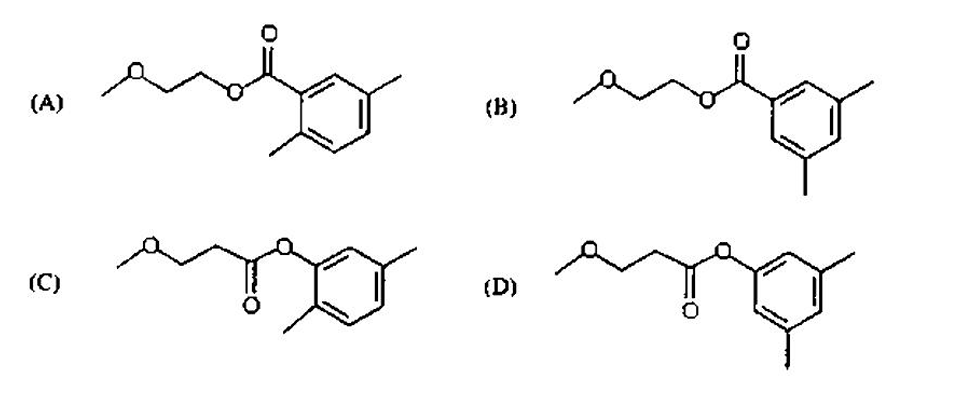
\includegraphics[width=0.75\linewidth]{figs/Q.50.png}
    \caption{fig23}
    \label{fig:figs/Q.50.png}
\end{figure}

\item The compound [Y] is
\hfill{GATE 2010 CY}
\begin{figure}[H]
    \centering
    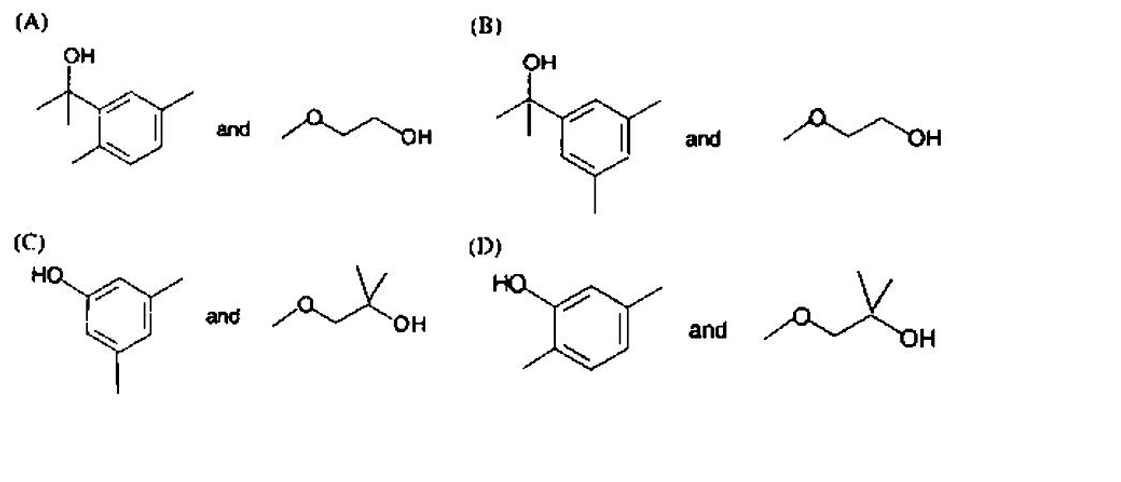
\includegraphics[width=0.75\linewidth]{figs/Q.51.png}
    \caption{fig24}
    \label{fig:figs/Q.51.png}
\end{figure}
statement for questions 52 and 53\\
\begin{figure}[H]
    \centering
    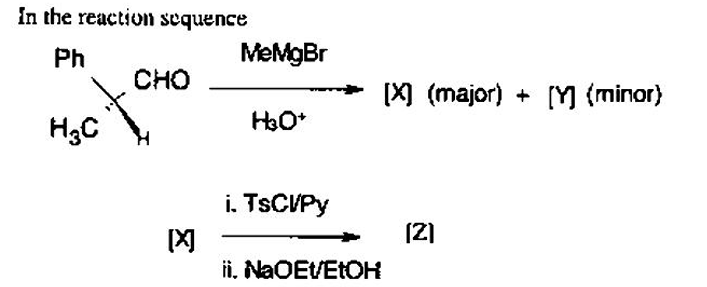
\includegraphics[width=0.75\linewidth]{figs/Q.52.1.png}
    \caption{fig25}
    \label{fig:figs/Q.52.1.png}
\end{figure}
\item 
the compound [X] is
\hfill{GATE 2010 CY}
\begin{figure}[H]
    \centering
    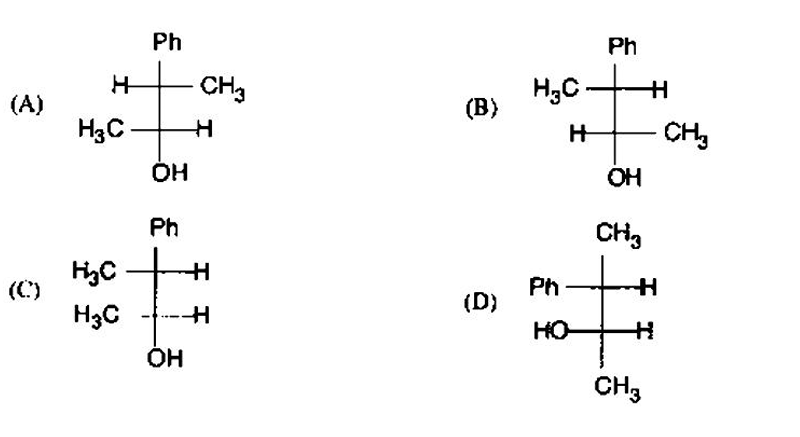
\includegraphics[width=1\linewidth]{figs/Q.52.2.png}
    \caption{fig26}
    \label{fig:figs/Q.52.2.png}
\end{figure}
\item 
the compound [Z] is
\hfill{GATE 2010 CY}
\begin{figure}[H]
    \centering
    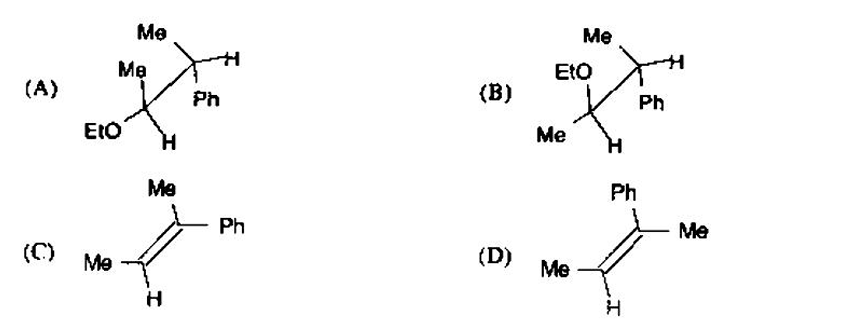
\includegraphics[width=1\linewidth]{figs/Q.53.png}
    \caption{fig27}
    \label{fig:figs/Q.53.png}
\end{figure}
Statements for linked questions 54 and 55\\
\begin{figure}[H]
    \centering
    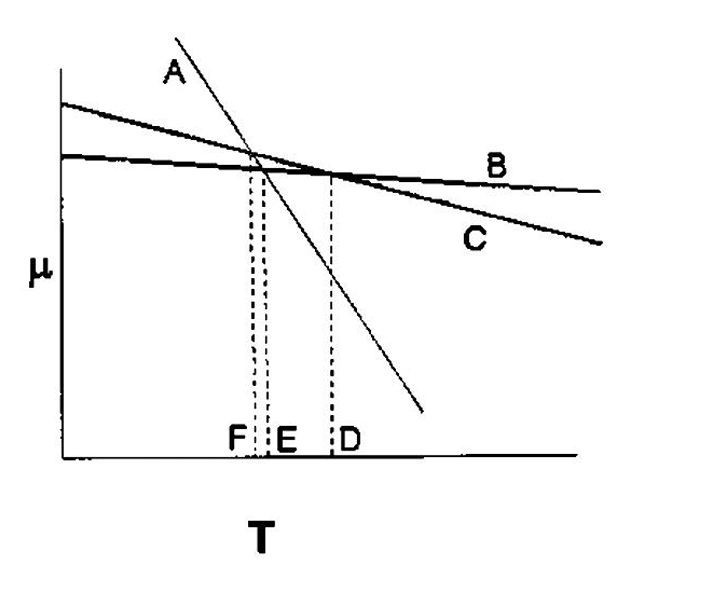
\includegraphics[width=0.75\linewidth]{figs/Q.54.png}
    \caption{fig28}
    \label{fig:figs/Q.54.png}
\end{figure}
\item Based on the above diagram:

\hfill{GATE 2010 CY}
\begin{multicols}{2}
\begin{enumerate}
    \item A represents the change in chemical potential as a function of temperature for the solid phase. B for the liquid and C for the gas
    \item A represents the change in chemical potential as a function of temperature for the liquid phase, B for the gas and C for the solid
    \item A represents the change in chemical potential as a function of temperature for the gas phase, B for the liquid and C for the solid
    \item A represents the change in chemical potential as a function of temperature for the gas phase, B for solid and C for the liquid
\end{enumerate}
\end{multicols}

\item From the same diagram

\hfill{GATE 2010 CY}
\begin{multicols}{2}
\begin{enumerate}
    \item D represents boiling point, E sublimation point and F melting point
    \item E represents boiling point, D sublimation point and F melting point
    \item E represents melting point, F sublimation point and D boiling point
    \item D represents melting point, F boiling point and E sublimation point
\end{enumerate}
\end{multicols}
General Aptitude Questions\\
56-60 carry one mark each
\item 25 persons are in a room. 15 of them play hockey, 17 of them play football and 10 of them play both hockey and football. Then the number of persons playing neither hockey nor football is:
\hfill{GATE 2010 CY}

\begin{multicols}{2}
\begin{enumerate}
    \item 2
    \item 17
    \item 13
    \item 3
\end{enumerate}
\end{multicols}

\item If we manage to \_\_\_\_\_\_\_ our natural resources, we would leave a better planet for our children.

\hfill{GATE 2010 CY}
\begin{multicols}{2}
\begin{enumerate}
    \item uphold
    \item restrain
    \item cherish
    \item conserve
\end{enumerate}
\end{multicols}

\item Unemployed : Worker

\hfill{GATE 2010 CY}
\begin{multicols}{2}
\begin{enumerate}
    \item fallow : land
    \item unaware : sleeper
    \item wit : jester
    \item renovated : house
\end{enumerate}
\end{multicols}

\item Circuitous

\hfill{GATE 2010 CY}
\begin{multicols}{2}
\begin{enumerate}
    \item cyclic
    \item indirect
    \item confusing
    \item crooked
\end{enumerate}
\end{multicols}
\item Choose the most appropriate word from the options given below to complete the following sentence:\\
His rather casual remarks on politics \rule{2cm}{0.15mm} his lack of seriousness about the subject.

\hfill{GATE 2010 CY}

\begin{multicols}{2}
\begin{enumerate}
    \item masked
    \item belied
    \item betrayed
    \item suppressed
\end{enumerate}
\end{multicols}
61-65 carry two marks each
\item Hari (H), Gita (G), Irfan (I) and Saira (S) are siblings (i.e., brothers and sisters). All were born on 1$^{\text{st}}$ January. The age difference between any two successive siblings (that is born one after another) is less than 3 years. Given the following facts:

\begin{itemize}
    \item[i.] Hari's age + Gita's age $>$ Irfan's age + Saira's age.
    \item[ii.] The age difference between Gita and Saira is 1 year. However, Gita is not the oldest and Saira is not the youngest.
    \item[iii.] There are no twins.
\end{itemize}

In what order were they born (oldest first)?

\begin{multicols}{2}
\begin{enumerate}
    \item HSGI
    \item SGHI
    \item IGSH
    \item IHSG
\end{enumerate}
\end{multicols}

\item 5 skilled workers can build a wall in 20 days; 8 semi-skilled workers can build a wall in 25 days; 10 unskilled workers can build a wall in 30 days. If a team has 2 skilled, 6 semi-skilled and 5 unskilled workers, how long will it take to build the wall?
\hfill{GATE 2010 CY}

\begin{multicols}{2}
\begin{enumerate}
    \item 20 days
    \item 18 days
    \item 16 days
    \item 15 days
\end{enumerate}
\end{multicols}

\item \textbf{Modern warfare has changed from large scale clashes of armies to suppression of civilian populations. Chemical agents that do their work silently appear to be suited to such warfare; and regretfully, there exist people in military establishments who think that chemical agents are useful tools for their cause.}\\
\textit{Which of the following statements best sums up the meaning of the above passage?}

\hfill{GATE 2010 CY}

\begin{multicols}{2}
\begin{enumerate}
    \item Modern warfare has resulted in civil strife.
    \item Chemical agents are useful in modern warfare.
    \item Use of chemical agents in warfare would be undesirable.
    \item People in military establishments like to use chemical agents in war.
\end{enumerate}
\end{multicols}

\item Given digits 2, 2, 3, 3, 3, 4, 4, 4, 4 how many distinct 4 digit numbers greater than 3000 can be formed?
\hfill{GATE 2010 CY}

\begin{multicols}{2}
\begin{enumerate}
    \item 50
    \item 51
    \item 52
    \item 54
\end{enumerate}
\end{multicols}

\item If 137 $+$ 276 $=$ 435 how much is 731 $+$ 672?
\hfill{GATE 2010 CY}

\begin{multicols}{2}
\begin{enumerate}
    \item 534
    \item 1403
    \item 1623
    \item 1513
\end{enumerate}
\end{multicols}

























































































    
\end{enumerate}







































\end{document}